\section{Generative Adversarial Networks (GANs)}
\label{sec:gan}

\begin{figure}
    \centering
    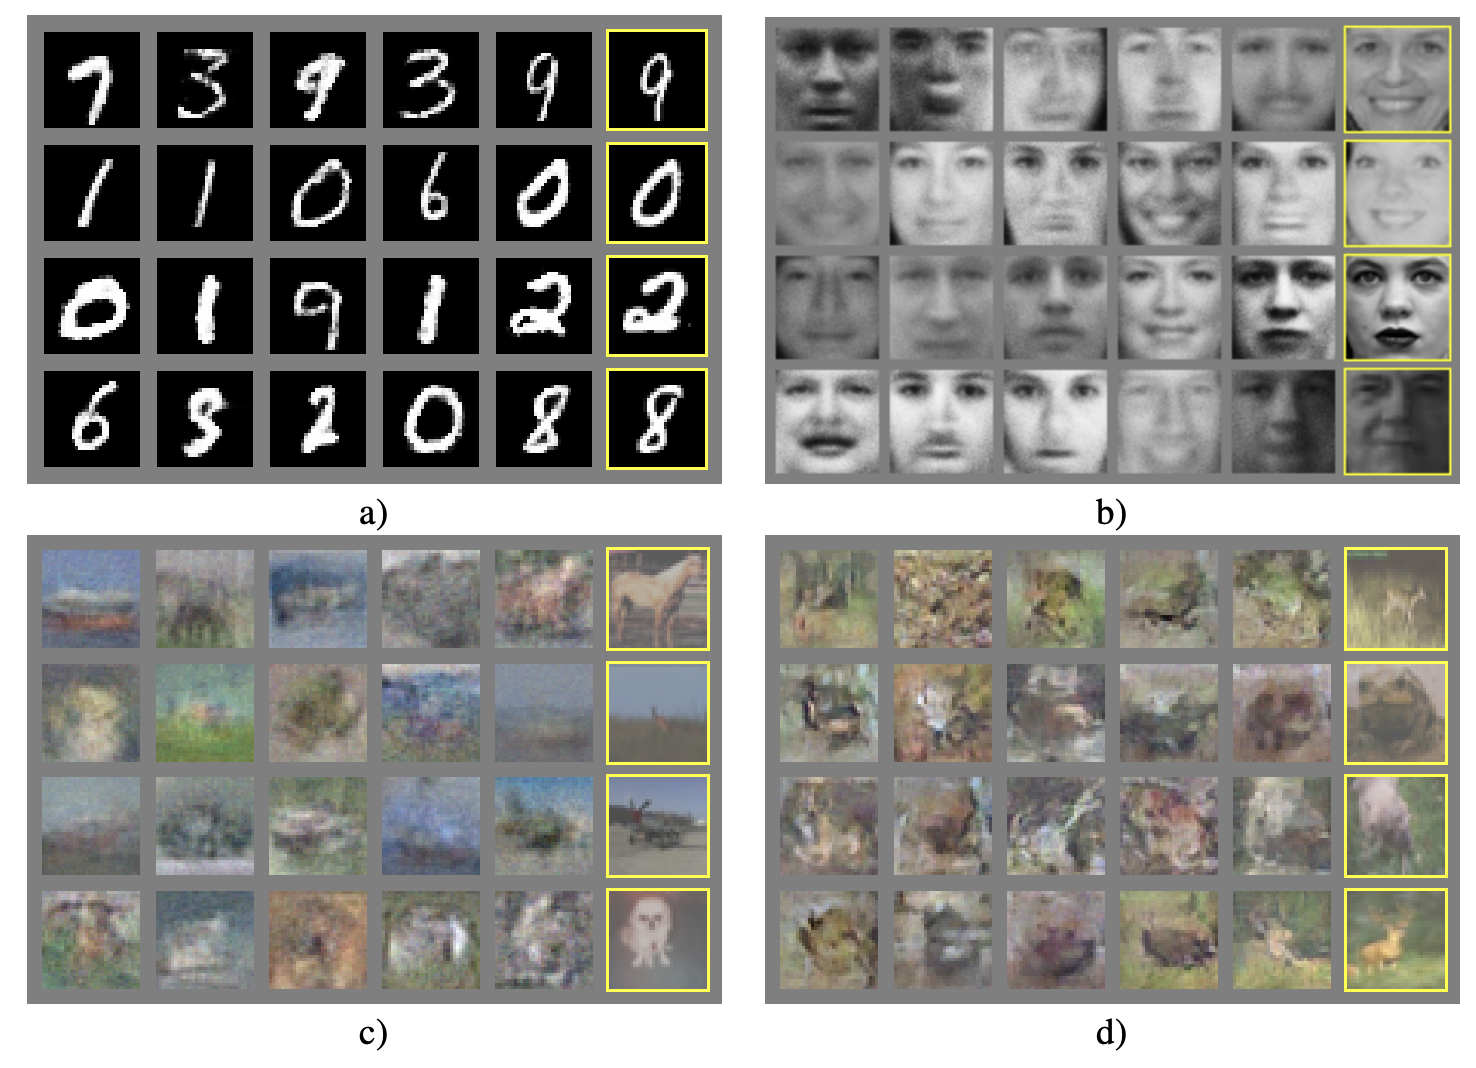
\includegraphics[width=0.75\textwidth]{images/gan/gan_samples.png}
    \caption{Some samples generated by GAN in the paper \cite{gan}. Right: samples from the training data. Left: samples generated by the model. a) is from the MNIST dataset, b) is from the Toronto Face Database (TFD), c) is from the CIFAR-10 dataset with fully-connected layers at the generator and discriminator, and d) is from the CIFAR-10 dataset with convolutional layers at the generator and discriminator.}
\end{figure}

Generative Adversarial Networks (GANs) \cite{gan} are a class of deep learning models that are used to generate new data samples from a given distribution. More specifically, they are very good at synthesizing high-quality images. The model can be used by itself, or as we will see later, it can also be the basis of other image and video generation models, such as VQ-GAN \ref{sec:vqgan}. The main breakthrough in this paper was the introduction of adversarial training and loss, which significantly improves the quality of generated images through a second model that judges the output images.

\begin{figure}
    \centering
    \resizebox{\textwidth}{!}{
        \begin{tikzpicture}
            % Real images, Generator nodes
            \node[rectangle, draw, fill=green!20, minimum width=2cm, minimum height=1cm] (real_images) {Real Images};
            \node[rectangle, draw, fill=red!20, minimum width=2cm, minimum height=1cm, below=of real_images] (generator) {Generator};

            % Noise node
            \node[rectangle, draw, fill=gray!20, minimum width=2cm, minimum height=1cm, left=of generator] (noise) {Noise};

            % Arrow from noise to generator
            \draw[->] (noise) -- (generator);

            % Sample nodes
            \node[rectangle, draw, fill=gray!20, minimum width=2cm, minimum height=1cm, right=of generator] (sample_gen) {Sample};
            \node[rectangle, draw, fill=gray!20, minimum width=2cm, minimum height=1cm, right=of real_images] (sample_real_images) {Sample};

            % Fit sample nodes in a box
            \node[fit=(sample_gen)(sample_real_images), inner sep=0] (sample_fitbox) {};


            % Arrows to sample nodes
            \draw[->] (real_images) -- (sample_real_images);
            \draw[->] (generator) -- (sample_gen);

            % Discriminator node
            \node[rectangle, draw, fill=blue!20, minimum width=2cm, minimum height=1cm, right=of sample_fitbox] (discriminator) {Discriminator};

            % Arrows to discriminator
            \draw[->] (sample_real_images) -- (discriminator);
            \draw[->] (sample_gen) -- (discriminator);

            % Discriminator loss, Generator loss
            % Matrix for the nodes to the right
            \matrix[
                right=of discriminator, 
                column sep=0.5cm, 
                row sep=0.5cm, 
                nodes={rectangle, draw, minimum width=4cm, minimum height=2cm, anchor=center}
            ] (matrix) {
                \node[rectangle, draw, fill=gray!20, minimum width=2cm, minimum height=1cm] (discriminator_loss) {Discriminator Loss}; \\
                \node[rectangle, draw, fill=gray!20, minimum width=2cm, minimum height=1cm] (generator_loss) {Generator Loss}; \\
            };

            % Add arrows
            \draw[->] (discriminator) -- (discriminator_loss);
            \draw[->] (discriminator) -- (generator_loss);
        \end{tikzpicture}
    }
    \caption{GAN architecutre \cite{gan}. Noise is sampled from a noise distribution and fed to the generator. The generator outputs an image, and the discriminator needs to decide if the image was generated by the generator or if its an image from the dataset. This decision then affects the value of the loss function, and the weights are updated accordingly by backpropogation.}
    \label{fig:gan_architecture}
\end{figure}

% Picture
\begin{figure}
    \centering
    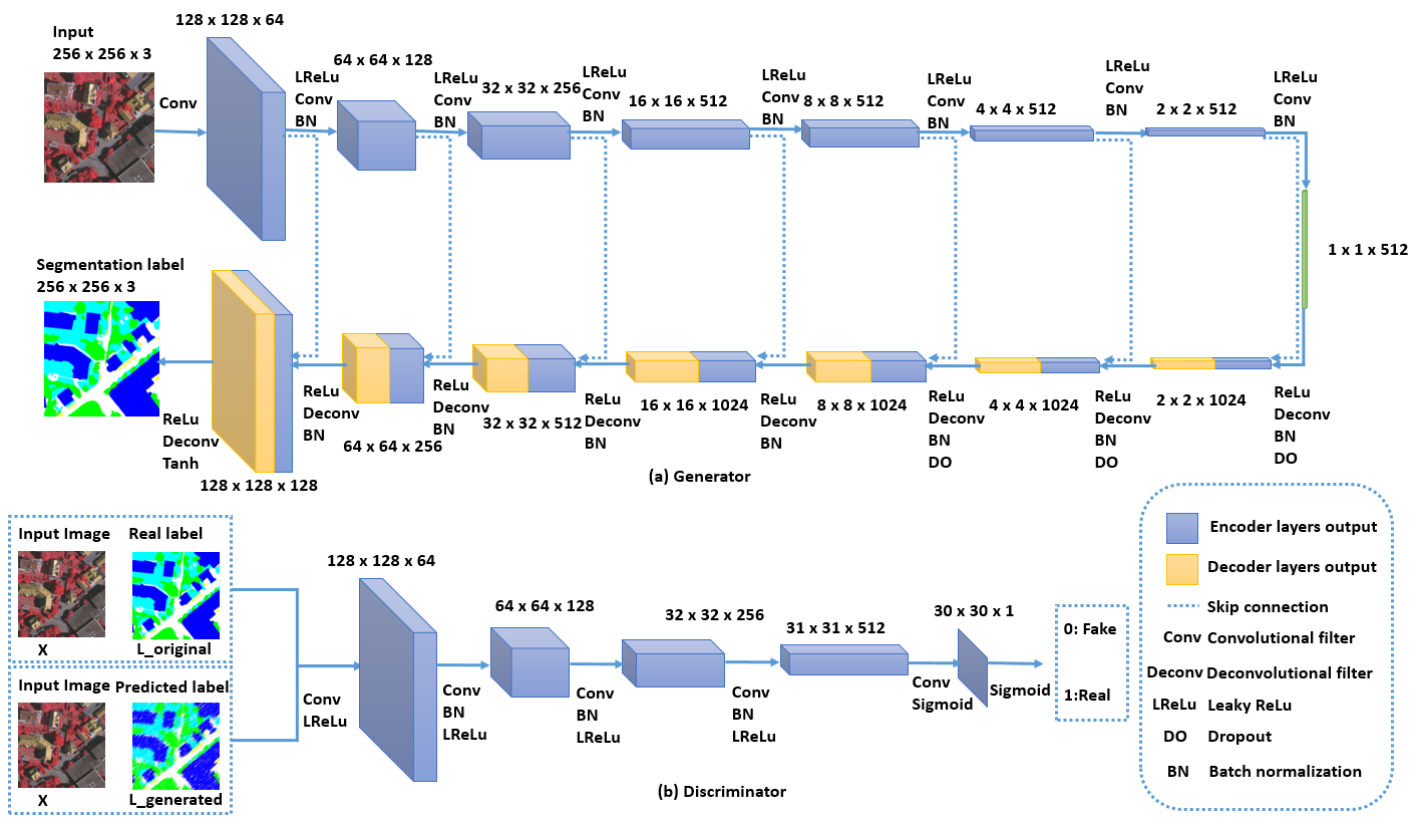
\includegraphics[width=0.8\textwidth]{images/gan/gan_architecture.png}
    \caption{More detailed architecture of GAN (from \cite{gan_architecture_figure_paper}). Its important to note that both the $G$ and $D$ networks are made up of multiple CNN layers (convolutional, deconvolution, fully connected and activation layers, such as relu, leaky relu, softmax and more). Softmax in $D$ indicates wether the image is real or fake (statistically 1 or 0).}
    \label{fig:gan_architecture}
\end{figure}

The model consists of two neural networks: a generator $G$ and a discriminator $D$ (as shown in figure \ref{fig:gan_architecture} and \ref{fig:gan_architecture_highlevel}). The generator is responsible for generating new samples $x$ (images), while the discriminator is responsible for distinguishing between real samples (from the dataset, $D(x) = 1$) and generated samples (fake, from the generator, $D(x) = 0$). The two networks are trained simultaneously in a minimax game (see training section \ref{subsec:gan_training}), where the generator tries to generate samples that are indistinguishable from real samples, and the discriminator tries to distinguish between real and generated samples. The training process continues until the generator is able to generate realistic and high-quality images. 

The noise vector is sampled from a simple distribution like Gaussian. A noise vector is simply a vector that each element in the vector is samples from a given distribution. The basic idea of using noise as input is that the model learns to establish relationships between each dimension in the vector and the output image, similar to latent vectors or code vectors. For instance, the model might learn that the first dimension of the noise vector corresponds to the shape of the middle of the image (like the shape of the head of a person), while the second dimension might corresponds to the color of the shape, and so on.

Because GANs don't use variational inference, like VQ-VAE, the model doesn't have control over the output image structure. Each noise vector will generate a different image. This problem created the need for conditional GANs, which future papers addressed to provide better control over the generated images by conditioning the model on additional information (see section \ref{subsec:gan_conditional_generation}).




\subsection{Training \& Adversarial loss}
\label{subsec:gan_training}

The loss function of the GAN model is defined as the following min-max game:

\begin{equation}
    \label{eq:gan_loss}
    \min_G \max_D V(D,G) = \mathbb{E}_{x \sim p_{\text{data}}(x)}[\log D(x)] + \mathbb{E}_{z \sim p_z(z)}[\log(1 - D(G(z)))]
\end{equation}

We have two prior distributions: $x \sim p_{\text{data}}$ and $z \sim p_z(z)$, where the noise vector $z$ is sampled from a noise distribution, and $p_{\text{data}}$ represents the true underlying distribution of the dataset, and $x$ is sampled from this distribution.

With respect to the discriminator gradients, the loss function tries to maximize the probability that:

\begin{enumerate}
    \item the discriminator correctly classifies real samples as real (the first term)
    \item the discriminator correctly classifies generated samples as fake (the second term)
\end{enumerate}


With respect to the generator gradients \footnote{When we do backpropogation with respect to the generator gradients, the first term is constant.}, the loss function tries to minimize the probability that:

\begin{enumerate}
    \item the generator tries to fool the discriminator in thinking that the generated samples are real (the second term)
\end{enumerate}


The researchers mentioned that at the beginning of the training, the discriminator rejects samples with high confidense. To address this, they suggested instead of \textbf{minimizing} the second term, to \textbf{maximize} a new second term in the loss function: $\log D(G(z))$.


\begin{figure}
    \centering
    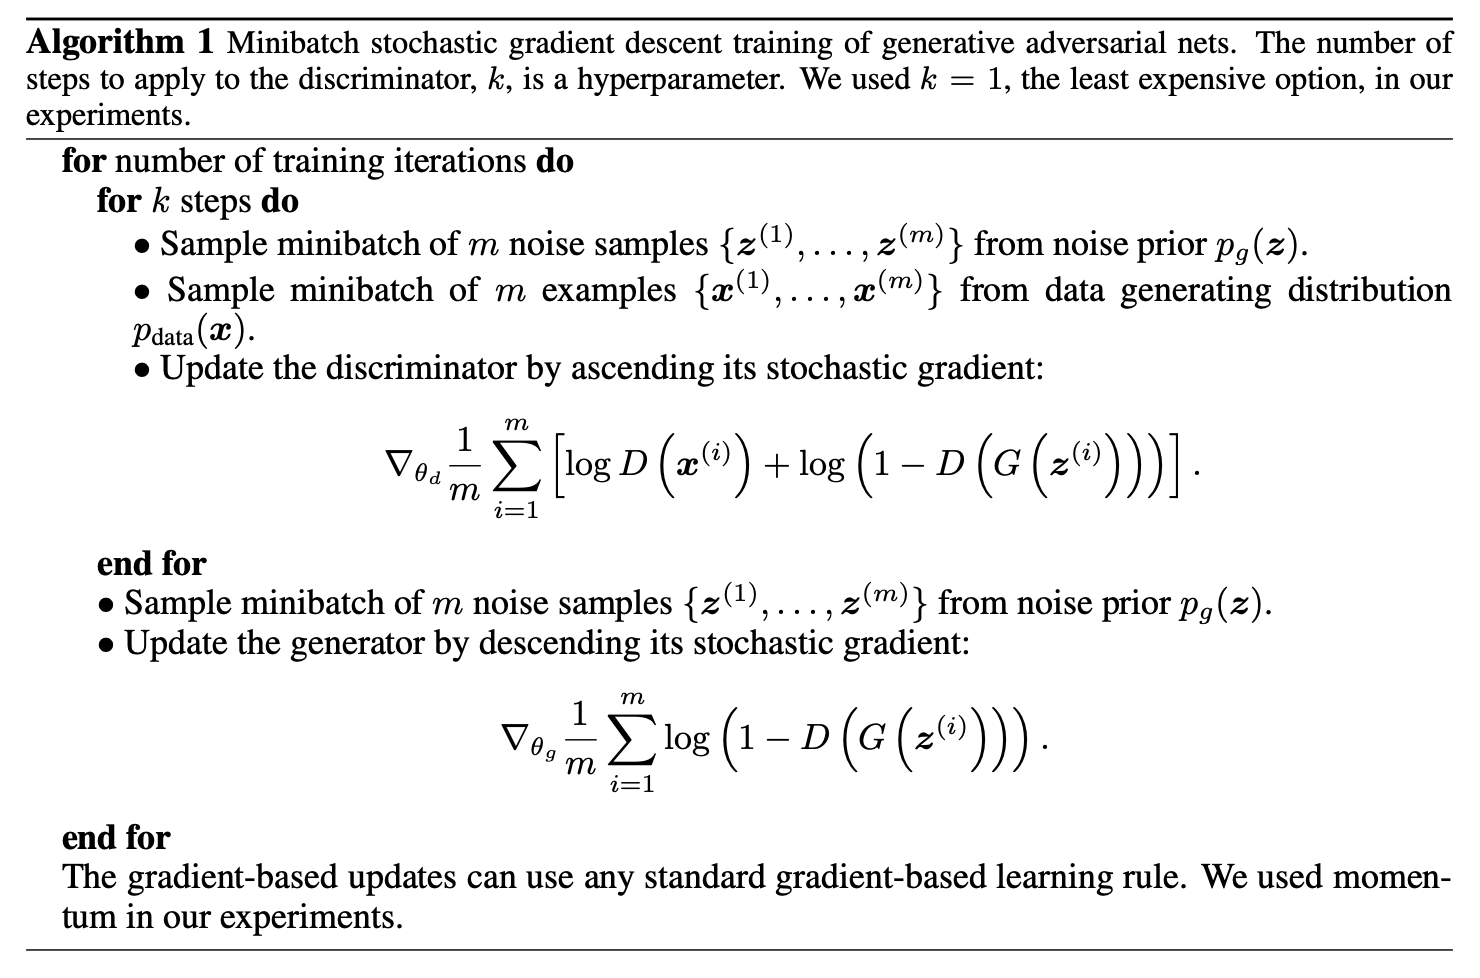
\includegraphics[width=0.8\textwidth]{images/gan/gan_training.png}
    \caption{The training algorithm for GAN using minibatch stochastic gradient decent \cite{gan}.}
    \label{fig:gan_training}
\end{figure}

In order to balance of the training for both $G$ and $D$ the authors suggested using iterative approach using minibatch stochastic gradient decent (see figure \ref{fig:gan_training}). Instead of fully optimizing $D$ in each iteration, the algorithm alternates between a few steps ($k$ steps) of optimizing the discriminator and one step of optimizing the generator. By updating $D$ more often the researchers hope to update the generator more slowly and stabilize the training process.



\subsection{Mode Collapse}
\label{gan_mode_collapse}

One of the main challenges of training GANs is mode collapse. Mode collapse occurs when the generator learns to generate only a few samples, instead of learning to generate a diverse set of samples. This can happen when the generator learns to generate samples that fool the discriminator, but failed to capture the full diversity of the training data distribution (see figure \ref{fig:gan_mode_collapse}). This can happen when the discriminator is too strong, and the generator is not able to generate diverse samples. In other words, the generator tries to fool the discriminator so much that it only focuses on this goal, while ignoring to diversify the samples.

\begin{figure}
    \centering
    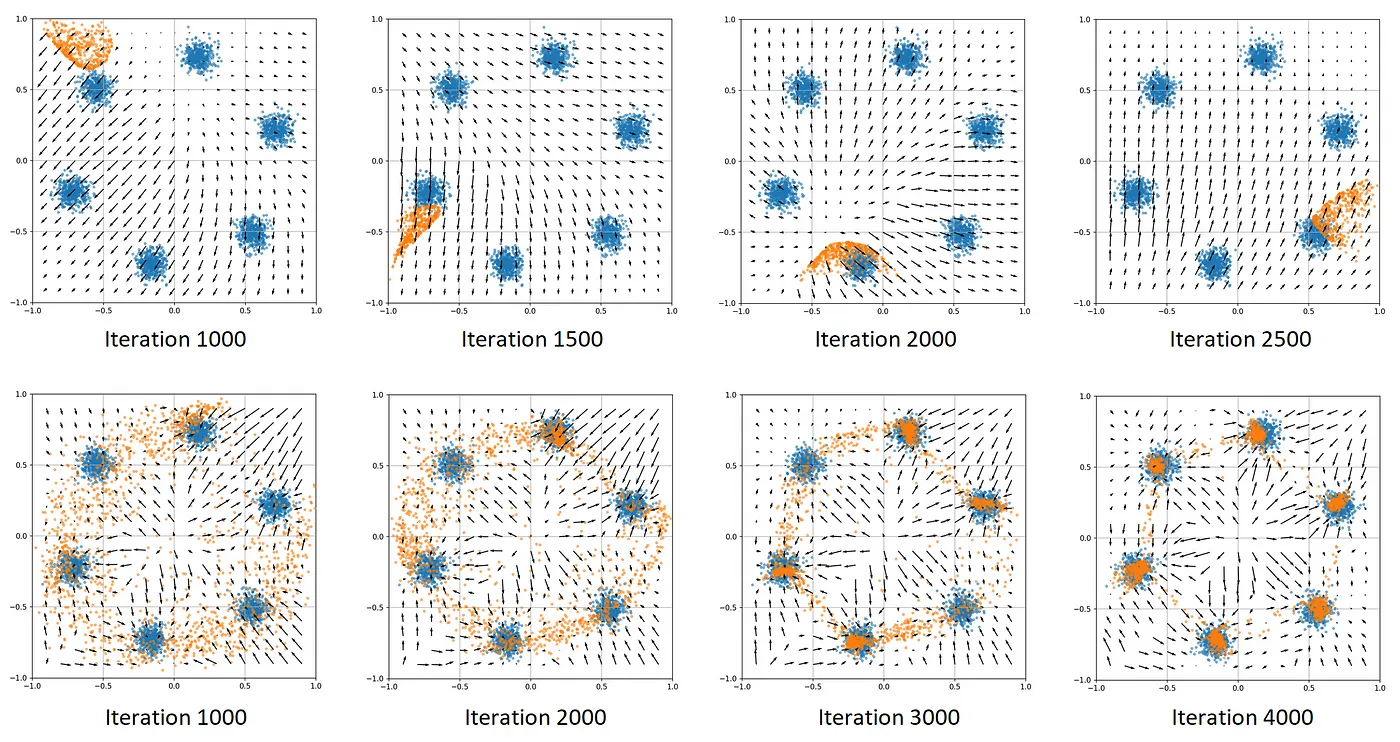
\includegraphics[width=\textwidth]{images/gan/gan_mode_collapse.png}
    \caption{Visualization of mode collapse in GANs \cite{gan_mode_collapse_image_source}. Top row shows the model failing to diversify its output, leading it to focus on specific mode of the dataset. Bottom row shows GAN samples without mode-collapse, where the model was successfully traind to diversify its output to match the underlying structure of the dataset. Blue dots are the prior $x \sim p_{\text{data}}(x)$ (the dataset) and the orange dots are the generated samples $p_g$.}
    \label{fig:gan_mode_collapse}
\end{figure}




\subsection{Conditional generation}
\label{subsec:gan_conditional_generation}

GANs produce realistic images but we can't choose the hair color, the pose, or background, without training seperate GANs for each combination of characteristics. Conditional generation models however do provide us with this control. Prominent conditional GAN models include: Conditional GAN (cGAN) \cite{cgan}, InfoGAN \cite{infogan}, CycleGAN \cite{cyclegan}, StyleGAN \cite{stylegan} and more, each with their own unique features and capabilities. For example, \textbf{StyleGAN} allows for the control of the style of the generated images by using a separate latent vector for each style. In \textbf{CycleGAN}, the model can learn to translate images from one domain to another without paired data. And in \textbf{InfoGAN}, the model can learn disentangled representations (called latent codes) of the data, which can be used to control the output of the generator (for example, one latent code might control the hair style, while another might control the hair color).

\begin{figure}
    \centering
    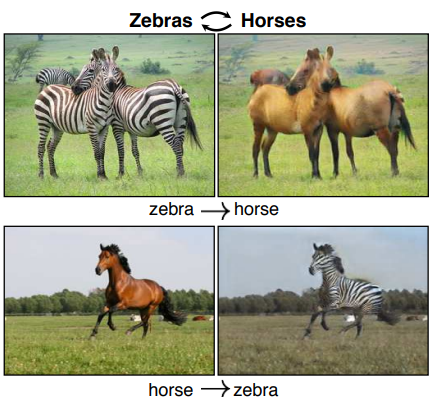
\includegraphics[width=0.35\textwidth]{images/gan/cyclegan.png}
    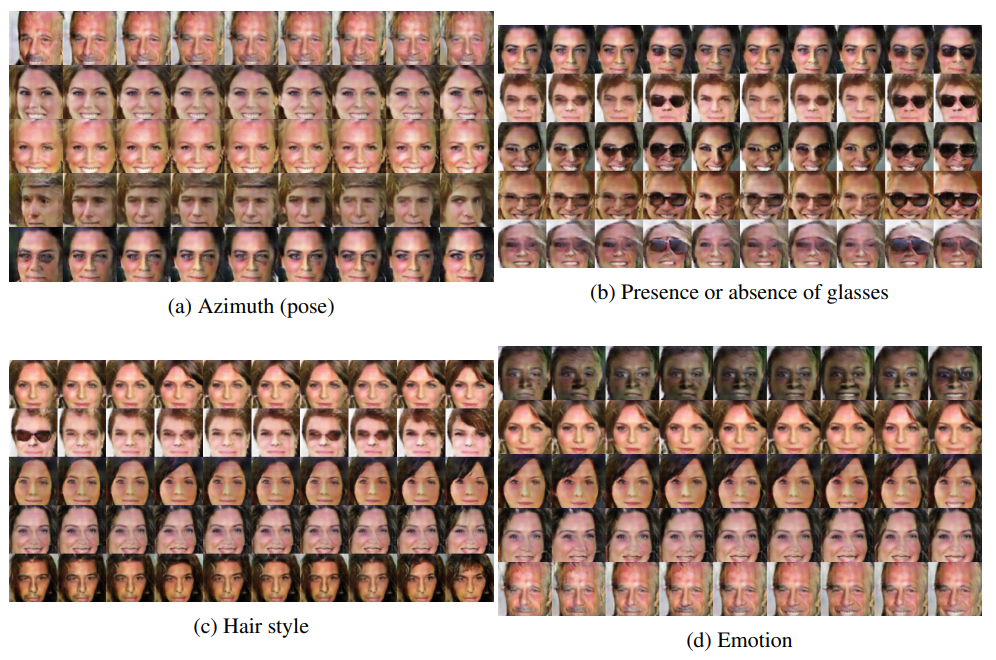
\includegraphics[width=0.6\textwidth]{images/gan/infogan.png}
    \caption{Left: CycleGAN can learn to automatically 'translate' an image from one into another and vice versa. Right: InfoGAN can learn disentangled representations of the data, which can be used to control the output of the generator. In this case, pose, glasses on face, hair style and emotion.}
\end{figure}

In the next sections we will take a look at different models with conditional capabilities.